\documentclass[12pt]{article}

\usepackage{graphicx}
\graphicspath{ {./images/} }
\begin{document}

Starting in calculus 3, we use 3d coordinate system rather than 2d.

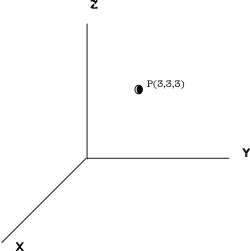
\includegraphics{3dgraph.png}

To form the graph, refer to the chart below.
\begin{quote}
	Point index to pinky finger in direction of 1; this shows the x-axis.
Then curl fingers towards 2 for the y-axis. The thumb indicates the z axis.	
\end{quote}

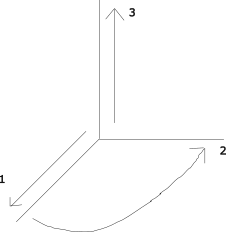
\includegraphics{howtomakegraph}

We use the \textbf{right hand rule} to get this (we use the right hand)\\
We can create a projection of a point onto xy, xz, yz plane by setting z, y, or x to 0. 

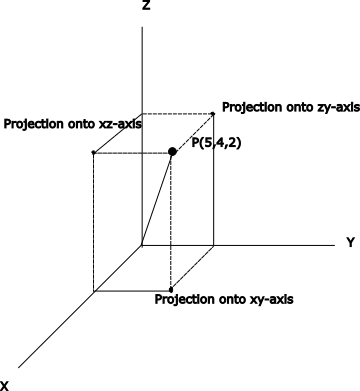
\includegraphics{projections-onto-3daxes}

Here the point P(5,4,2) is plotted and the projections onto the 3 planes are displayed.
From left to right: (0,4,2), (5,0,2), (5,4,0)

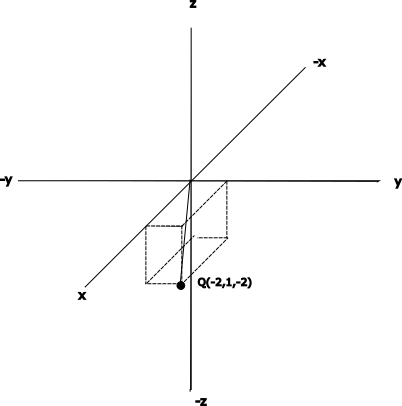
\includegraphics{projection2}

The graph above demonstrates a point Q(2,1,-2) where the x coordinates are now negative.
An error was made where the x coordinate in the graph is negative when it is in fact positive.

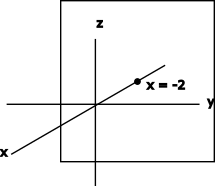
\includegraphics{parallelzy}
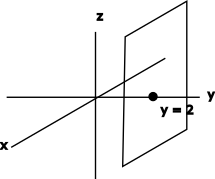
\includegraphics{parallelxz}

The preceding graphs demonstrate planes parallel to the zy and xz planes respectively. 
Notice for each of the graphs, there is a single fixed point and domains for unfixed coordinates are $\in{R}$.


\end{document}

